\chapter{Overleaf \\
\small{\textit{-- Annanya Jain, Luo Xu, Gavin Lam}
\index{Overleaf} 
\index{Chapter!Overleaf}
\label{Chapter::Overleaf}}}

\title{Deploying Overleaf on a Shared DigitalOcean Droplet (with Existing Bugzilla)}
\section{Overview}
TThis document explains the complete process of deploying \textbf{Overleaf (Community Edition)} on a DigitalOcean droplet that already hosted \textbf{Bugzilla} via Docker.  
It includes the initial access issues, configuration steps, and debugging process that led to a fully functional Overleaf instance running alongside Bugzilla on the same host.

\section{Initial Access Issue}
At the beginning, I could not connect to the droplet from my local machine using its public IP address.  
Both \texttt{ssh root@174.138.68.199} and web requests to \texttt{http://174.138.68.199} were failing with timeout errors.

Since I didn’t originally create the droplet, I did not have SSH access permissions. To resolve this, my teammate who had created the droplet and had root access, added my GitHub SSH key to the droplet’s authorized keys through the DigitalOcean dashboard:

\begin{enumerate}
  \item Logged into \textbf{DigitalOcean}.
  \item Opened the droplet’s page.
  \item Navigated to \textbf{Access → Add SSH Keys}.
  \item Added my GitHub SSH key (fetched automatically from my GitHub account).
\end{enumerate}

After this, I was able to connect successfully:
\begin{minted}[fontsize=\small]{bash}
ssh root@174.138.68.199
\end{minted}

Once connected, I could verify that Bugzilla was already running:
\begin{minted}[fontsize=\small]{bash}
docker ps
\end{minted}

Bugzilla was occupying port 80, so I decided to host Overleaf on a different port.

\section{Overleaf Setup Process}

\subsection{Step 1: Create Project Directory}
\begin{minted}[fontsize=\small]{bash}
mkdir ~/overleaf-docker
cd ~/overleaf-docker
\end{minted}

\subsection{Step 2: Create Environment File}
\begin{minted}[fontsize=\small]{bash}
nano .env
\end{minted}

Contents:
\begin{minted}[fontsize=\small]{text}
OVERLEAF_PORT=8090
OVERLEAF_DOMAIN=http://174.138.68.199:8090
OVERLEAF_ADMIN_EMAIL=(email here)
OVERLEAF_ADMIN_PASSWORD=(password here)
MONGO_INITDB_ROOT_USERNAME=(username here)
MONGO_INITDB_ROOT_PASSWORD=(password here)
\end{minted}

\subsection{Step 3: Write the Docker Compose File}
\begin{minted}[fontsize=\small, bgcolor=gray!5, linenos]{yaml}
version: "3.8"

services:
  mongo:
    image: mongo:6.0
    restart: unless-stopped
    command: ["--replSet", "rs0", "--bind_ip_all"]
    volumes:
      - mongo_data:/data/db

  redis:
    image: redis:7
    restart: unless-stopped

  overleaf:
    image: sharelatex/sharelatex:latest
    restart: unless-stopped
    depends_on:
      - mongo
      - redis
    ports:
      - "8090:80"
    environment:
      OVERLEAF_MONGO_URL: mongodb://mongo:27017/sharelatex?replicaSet=rs0
      OVERLEAF_REDIS_HOST: redis
      OVERLEAF_SITE_URL: http://174.138.68.199:8090
      OVERLEAF_ADMIN_EMAIL: admin@example.com
      OVERLEAF_ADMIN_PASSWORD: password123
      OVERLEAF_APP_NAME: Overleaf
      OVERLEAF_ALLOW_PUBLIC_REGISTRATION: "true"

volumes:
  mongo_data:
\end{minted}


\subsection{Step 4: Launch the Containers}
\begin{minted}[fontsize=\small]{bash}
docker compose up -d
docker ps
\end{minted}

At this point, MongoDB, Redis, and Overleaf containers appeared, but Overleaf was continuously restarting.

\section{Debugging the Overleaf Restart Loop}

\subsection{Step 1: Check Logs}
\begin{minted}[fontsize=\small]{bash}
docker logs overleaf-docker-overleaf-1 --tail 40
\end{minted}

\subsection{Step 2: Error Observed}
\begin{minted}[fontsize=\small]{text}
The MongoDB server has featureCompatibilityVersion=5.0,
but Overleaf requires at least version 6.0.
Aborting.
\end{minted}

\begin{figure}
    \centering
    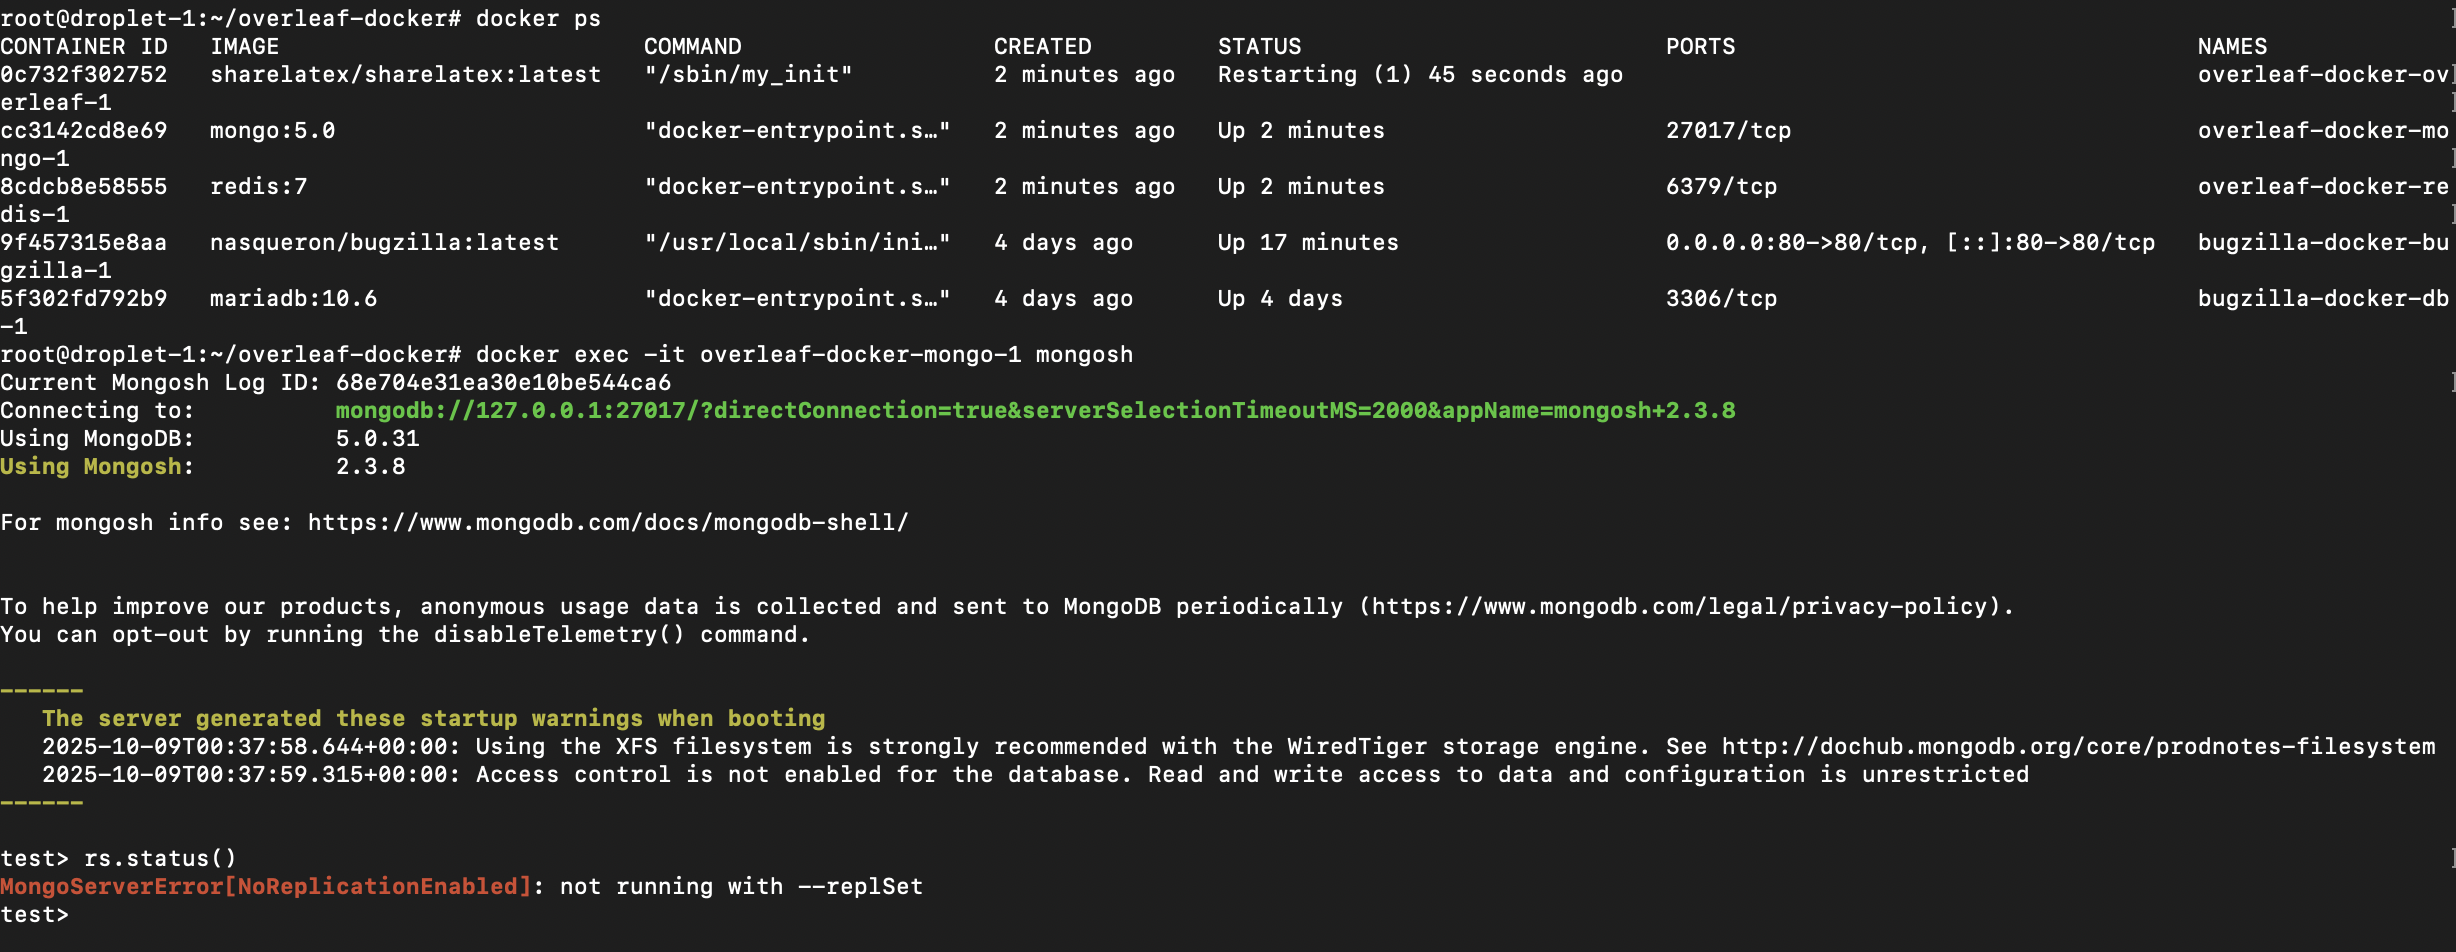
\includegraphics[width=1.0\linewidth]{png/restarting_problem_overleaf.png}
\end{figure}

This indicated that MongoDB was version 6.0, but its internal
\texttt{featureCompatibilityVersion (FCV)} was still set to 5.0.

\section{Fixing MongoDB Configuration}

\subsection{Step 1: Enter Mongo Shell}
\begin{minted}[fontsize=\small]{bash}
docker exec -it overleaf-docker-mongo-1 mongosh
\end{minted}

\subsection{Step 2: Initialize Replica Set}
\begin{minted}[fontsize=\small]{js}
rs.initiate()
\end{minted}

If you see \texttt{MongoServerError[AlreadyInitialized]}, it means it’s already set up — that’s fine.

\subsection{Step 3: Update Feature Compatibility Version}
\begin{minted}[fontsize=\small]{js}
use admin
db.adminCommand({ setFeatureCompatibilityVersion: "6.0" })
\end{minted}

Expected output:
\begin{minted}[fontsize=\small]{json}
{ "ok" : 1 }
\end{minted}

\subsection{Step 4: Restart Overleaf}
\begin{minted}[fontsize=\small]{bash}
exit
docker restart overleaf-docker-overleaf-1
\end{minted}


\section{Making Overleaf Publicly Accessible}

Since Bugzilla was already bound to port 80, Overleaf was assigned to port 8090.  
I confirmed the port was open:
\begin{minted}[fontsize=\small]{bash}
ss -tuln | grep 8090
\end{minted}

Then enabled it in the firewall:
\begin{minted}[fontsize=\small]{bash}
sudo ufw allow 8090/tcp
sudo ufw reload
\end{minted}

\section{Access and Verification}
Once restarted, Overleaf was reachable at:
\begin{minted}[fontsize=\small]{text}
http://174.138.68.199:8090
\end{minted}

I verified it via:
\begin{minted}[fontsize=\small]{bash}
curl -I http://174.138.68.199:8090
\end{minted}

Result:
\begin{minted}[fontsize=\small]{text}
HTTP/1.1 200 OK
\end{minted}

\section{Conclusion on Setting up Overleaf}
The deployment succeeded after:
\begin{enumerate}
  \item Gaining SSH access by adding my GitHub SSH key to the droplet.
  \item Running Overleaf on port 8090 (to avoid conflict with Bugzilla on port 80).
  \item Initializing the MongoDB replica set.
  \item Updating the MongoDB feature compatibility version to 6.0.
\end{enumerate}

After these steps, Overleaf was fully functional and accessible publicly via:
\begin{minted}[fontsize=\small]{text}
http://174.138.68.199:8090
\end{minted}

\begin{figure}
    \centering
    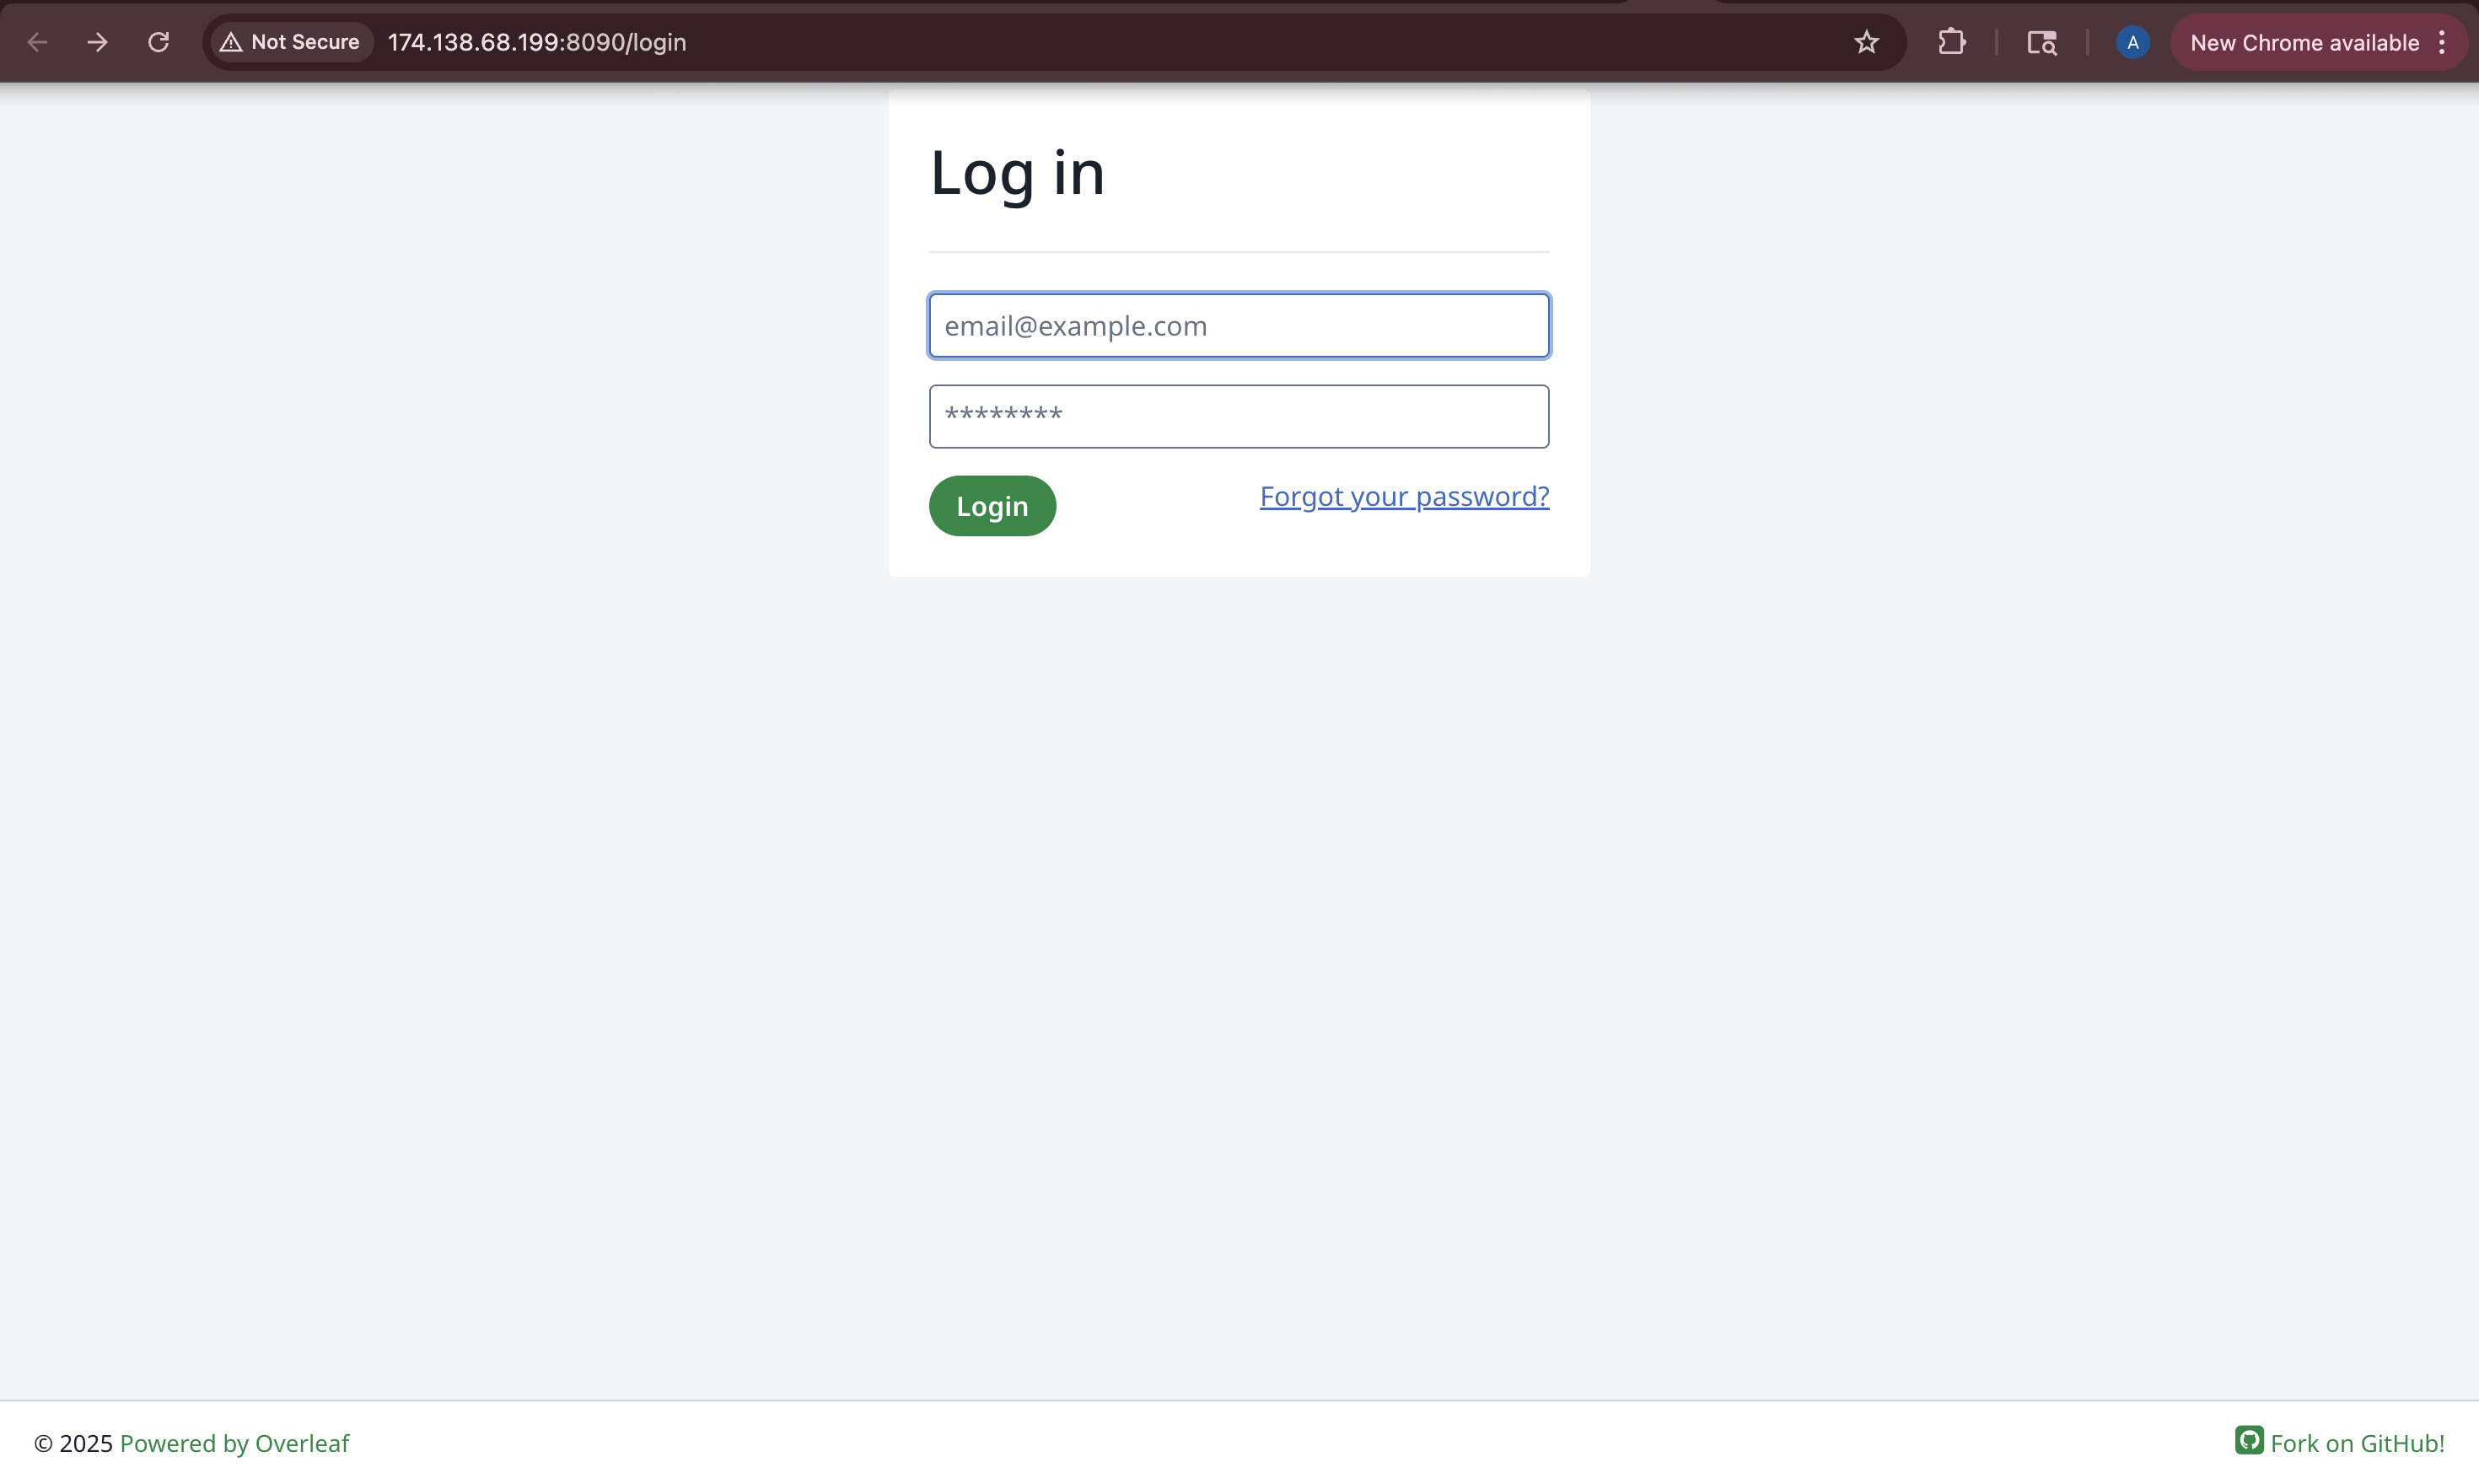
\includegraphics[width=1.0\linewidth]{png/overleaf running.png}
    \caption{overleaf website on http://174.138.68.199:8090}
    \label{fig:placeholder}
\end{figure}

This was what was seen:
\begin{figure}
    \centering
    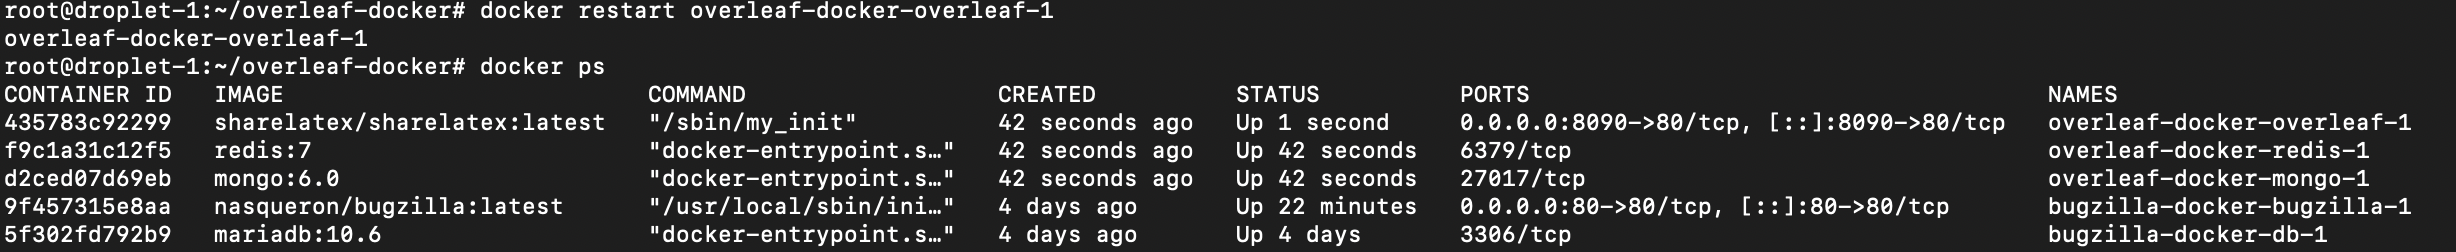
\includegraphics[width=1.0\linewidth]{png/finally_fixed.png}
\end{figure}

\section{Setting up Overleaf Packages}
Even thought Overleaf is up and running, we weren't able to run our document due to Overleaf not having access to any of the packages we were using. Thus we had to download the packages needed with commands:
\begin{minted}{bash}
apt-get update
apt-get install -y texlive-full
mktexlsr
\end{minted}
This took a long time to run, but afterwards our notebook was able to compile and had no errors in showing the pdf, however minted has refused to work even after installation...

\section{Connection Our Overleaf Instance to GitHub}
I first created a new GitHub Repository to for Overleaf, and then connected to our droplet. I downloaded the zip file for the Overleaf, then I copied it over to the vm and unzipped it under the repo. 